\section{The \Mesh Allocator}
\label{sec:allocator}



\Mesh is a memory allocator and runtime system for Linux that provides
a drop in replacement for the standard C/C++ and POSIX allocation
functions available from libc.  Mesh can be explicitly linked against,
e.g. by passing \texttt{-lmesh} to the linker at compile time, or used
with \texttt{LD\_PRELOAD} by the dynamic linker at execution time.
When loaded, \Mesh \textit{interposes} on calls to standard libc
functions, providing alternative functionality (in the case of
\texttt{malloc}) or to do bookkeeping before invoking libc's
implementation (in the case of \texttt{pthread\_create}.

\begin{figure}
  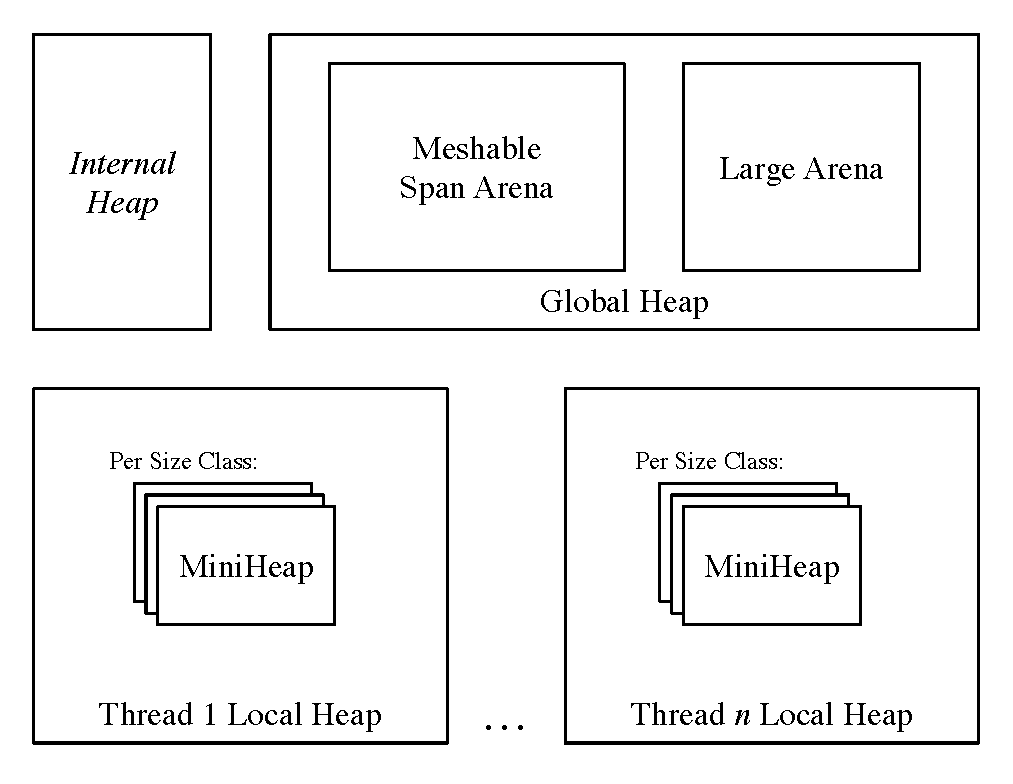
\includegraphics[width=.5\textwidth]{figures/global_heap}
  \caption{The allocator in mesh is managed by 4 main components.  The
    internal allocator provides management for \Mesh-internal dynamic
    data structures.  The global heap manages both the meshable arena
    spans are allocated out of, along with large objects.  Each thread
    has a local heap which satisfies small allocations from MiniHeaps,
    where there is one MiniHeap per size class.}
  \label{fig:global-heap}
\end{figure}

Mesh has three main components: the \textit{global heap} and runtime
state shared by all threads, \textit{thread local heaps} that can
satisfy allocations without taking locks, and MiniHeaps to track
occupancy and other metadata for spans.

Mesh is segregated-fit allocator.  Allocations are fulfilled from the
smallest size class they fit in (e.g. objects of size 32-64 bytes),
and objects larger than 16 KiB are individually served from the large
allocation region.

Spans, introduced in Section~\ref{sec:meshing}, are multiples of the
page size and contains between 8 and 256 objects of a constant size.

\subsection{MiniHeaps}

Miniheaps manage allocated physical spans of memory.  Each MiniHeap
contains metadata on the span start address and length, object size,
and allocation bitmap.  The number of objects that can be allocated
out of this bitmap is the \textit{objectCount = spanSize / objSize}.
The allocation bitmap is initialized to \textit{objectCount} zero
bits, and when an object is allocated the bit corresponding to its
offset from the start of the span is set to one.  Bitmap operations
are atomic, in order to ensure consistency without locking in
multi-threaded programs.

When a MiniHeap is allocated, there is a single virtual span that
points to the physical memory managed by the MiniHeap, and this
virtual span corresponds to the identity mapping between virtual and
physical offsets in the meshing arena.  After meshing there may be
multiple virtual spans that point to the MiniHeaps physical memory.

Miniheaps are either in-use or detached.  An in-use MiniHeap is owned
by a single local heap, while a detached MiniHeap is only referenced
by the global heap.  New objects are \textit{only} allocated out of
in-use MiniHeaps, and each in-use MiniHeap has an associated shuffle
freelists that is used to ensure fast randomized allocation.

\subsubsection{Shuffle Freelists}

\begin{figure}[!ht]
  \input{./local-malloc.cc}
  \input{./miniheap-malloc.cc}
  \input{./local-free.cc}
  \input{./miniheap-free.cc}
  \caption{Pseudocode for mesh allocation and deallocation routines.}
  \label{fig:malloc}
\end{figure}

In order to allocate objects randomly from a span in constant time, we
maintain a per-thread freelist of object offsets.  These offsets are
from the start of the span:

\vspace{-1.2em}
\begin{align*}
  \text{\textit{ptr}} = \text{\textit{spanStart + off*objSize}}
\end{align*}

This freelist is initialized with all of the available offsets $[0
  .. $ objectCount $]$ and then sorted with the Knuth-
Fischer-Yates shuffle~\cite{knuth:1981:semi}.

When an object is freed and the owning MiniHeap is still in-use, a
single iteration of the shuffle is performed to re-add the newly freed
offset back to the list of available offsets.

\begin{figure}[!t]
  \begin{subfigure}[t]{.4\textwidth}
    \centering
    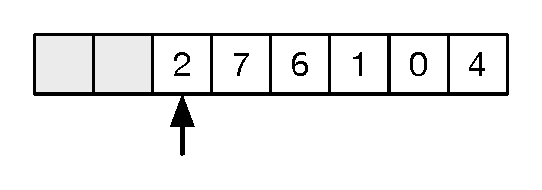
\includegraphics[width=\textwidth]{figures/shuffle-freelist_a}
    \caption{A freelist for a span of size 8, where 2 objects have
      already been allocated.}
  \end{subfigure}%
  ~

  \begin{subfigure}[t]{.4\textwidth}
    \centering
    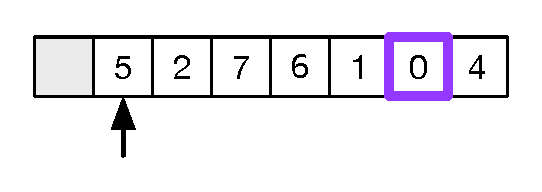
\includegraphics[width=\textwidth]{figures/shuffle-freelist_b}
    \caption{The offset is pushed on the front of the list, the list
      head pointer is updated, and a random element in [1,7] is chosen
      to swap with.}
  \end{subfigure}%
  ~

  \begin{subfigure}[t]{.4\textwidth}
    \centering
    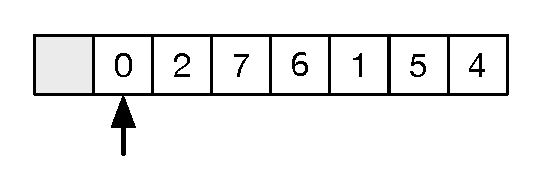
\includegraphics[width=\textwidth]{figures/shuffle-freelist_c}
    \caption{After the swap happens, new allocations proceed in a
      bump-pointer-like fashion.}
  \end{subfigure}
  \caption{Shuffle freelists enable bump-pointer-like random
    allocation out of a span.  When an object is freed and the
    MiniHeap it was allocated from is still attached to the local
    thread, its offset (5, in this example) is added back to the
    freelist with a single re-shuffle.}
  \label{fig:shuffle-freelists}
\end{figure}

Shuffle freelists are used in place of the random probing approach
used in Diehard and
Dieharder~\cite{1134000,Novark:2010:DSH:1866307.1866371}.  Random
probing works by choosing a random number in
$[0,\text{\textit{objectCount}}-1]$ and if that bit is zero in the
bitmap, setting it to one and using it as the offset for allocation.
If the offset is already one, a new random offset is chosen and the
process repeated.  Random probing allocates objects in $O(1)$ expected
time, with the catch that it requires overprovisioning memory.
Shuffle freelists solve this problem and provide $O(1)$ allocations
and frees not only in expectation, and with lower constants.

With maximum of 256 objects in a span, each offset in the freelist can
be represented as an unsigned character.  As we only need a freelist
for in-use MiniHeaps, the amount of memory required for freelists is
$256ct$, where $c$ is the number of size classes (11 in the current
implementation) and $t$ is the number of live threads, about 2.8 KiB
per thread.

\subsubsection{Locality}

Shuffle freelists give \Mesh bump-pointer like allocation speed in the
common case.  Like DieHard but unlike many other allocators, \Mesh
does not try to allocate consecutive objects nearby.  Modern 64-bit
Intel processors have 64-byte cache-lines, and ARM devices have 32 or
64-byte cache lines, meaning that object locality has little impact on
L1 cache locality.  TLB pressure should be unaffected compared to
other segregated-fit allocators with the same choice of size classes,
as for small objects we allocate randomly within a 4-KiB span, which
matches the page size.

\subsection{Thread Local Heap}

All malloc and free requests are initially handled by the thread local
heap.  The thread local heap has pointers to MiniHeaps for each size
class, a reference to the global heap, and its own random number
generator.

For small object allocations, the requested object size is converted
into a size class.  There is either an attached MiniHeap for that size
class, or a new one is requested from the global heap.  If after
allocating an object a MiniHeap is full (the freelist associated with
that MiniHeap is empty), the freelist is freed and the MiniHeap
detached from the local heap.  A new MiniHeap will be allocated the
next time an object of that size class is requested.

If the allocation request is for a large object (larger than 16 KiB),
it is forwarded on to the global heap.  Otherwise, the MiniHeap
corresponding to the size-class of the request is

A free request is either for an object in a span owned by an attached
MiniHeap, or forwarded to the global heap.

\subsection{Global Heap}

The global heap allocates new MiniHeaps for thread-local heaps,
handles all large object allocation and deallocation, performs
non-local frees for all objects, and coordinates meshing.

\subsubsection{MiniHeap allocation}

The global heap has an arena that meshable spans are allocated out of.
It is managed with a combination of a bitmap for tracking allocated
\textit{pages}, a red-black tree for retrieving the MiniHeap
corresponding to a pointer in $O(\lg{n})$ time, where $n$ is the heap
size, and per-size-class linked lists of all live MiniHeaps.

Allocating a MiniHeap involves reserving a set of $k$ consecutive
pages in the arena bitmap, allocating and initializing a new MiniHeap
instance from \Mesh's internal allocator, initializing the MiniHeap's
shuffle freelist, and recording the MiniHeap in the global red-black
tree and size-class-specific linked list.

\subsubsection{Large objects}

Large objects are allocated directly as anonymous \texttt{mmap}
mappings and returned to the OS on free with \texttt{munmap}.

As large objects are many multiples of the page size, they do not
suffer from fragmentation.

\subsubsection{Non-local frees}

If \texttt{free} is called on a pointer that does not belong to that
thread's local heap, the free is handled by the global heap.  A
read-lock is obtained, the MiniHeap is looked up in the global heap's
red-black tree of all MiniHeaps and that MiniHeap's bitmap is updated
atomically in a compare-and-set loop.

There are two reasons non-local frees may happen: enough objects of
the object's size class have occurred on the current thread that the
parent MiniHeap was exhausted and detached, or the pointer was
allocated on a remote thread.

\subsection{Meshing}

The \Mesh implementation is guided by the results in
Section~\ref{sec:meshing} to find a number of spans that can be meshed
together.

Non-local frees to the global heap initiate the meshing process with
low probability.  The reason only non-local frees may initiate a mesh
check is that frees that are able to be handled thread-locally can not
be contributing towards fragmentation, so they do not need to take a
chance that they will have to spend significant time attempting to
defragment the entire heap.  After a uniformly distributed random
number of non-local frees in, say, $[0,10000]$ has elapsed, meshing is
attempted.

We find meshes with heuristics, which is currently the
shuffle-neighbor approach described in Section~\ref{sec:heuristics}.

Meshing proceeds one size-class at a time, as each size-class is an
independent instance of the meshing problem.  Found meshes are
recorded in a list, to be batch applied at once.

Meshing spans together is a two step process: objects must be first
consolidated onto a single physical span before the process's
virtual-to-physical mapping is updated to point all meshed virtual
spans at the consolidated physical span.

Consolidating objects is a straightforward process of copying the
memory of objects from one span into free space of the other span, and
combining MiniHeap metadata (like the allocation bitmap).
Importantly, as \Mesh copies data at the physical span layer, even
though objects are moving in memory, no pointers or data internal to
moved objects or external references needs to be updated.

\subsubsection{Stop the World}

Object copying happens during a stop-the-world pause where all program
threads are halted.  If object consolidation were allowed to run
concurrently with application code it would expose a race condition
where the program could write to the original object after it was
copied but before the virtual to physical mapping was up to date.
These writes would then be lost when the page tables were updated,
causing serious, intermittent and hard to diagnose crashes.

This stop the world pause is implemented through careful use of
signals, signal handlers and condition variables.

\subsubsection{Page Table Updates}

Updating the process's page tables is done with calls to
\texttt{mmap}.  We exploit the fact that mmap allows the same offset
in a file (corresponding to a physical span) to be mapped to multiple
addresses.  Our small object arena, rather than being an anonymous
mapping, is a mapping backed by a temporary file.  This temporary file
is obtained through the \texttt{memfd\_create} system call and never
exists on the filesystem, only in memory.

Once objects are copied and the process's page tables are updated, all
application threads are unblocked and resume execution.
